\documentclass{article}
\usepackage{indentfirst}
\usepackage{graphicx}
\usepackage{algorithmicx}
\usepackage{subcaption}
\usepackage[outputdir=tex-output, cachedir=tex-output]{minted}
\usepackage[a4paper, total={170mm,257mm}, left=20mm, top=20mm]{geometry}

\usepackage{hyperref}
\hypersetup{
    colorlinks=true,
    linkcolor=blue,
    filecolor=magenta,      
    urlcolor=cyan,
    pdftitle={Overleaf Example},
    pdfpagemode=FullScreen,
}
\urlstyle{same}


\usepackage[backend=biber, style=ieee]{biblatex}
\addbibresource{ref.bib}

\usepackage{fancyhdr}
\pagestyle{fancy}
\fancyhf{}
\newenvironment{newSec}[1]{
	\section{#1}
	\lhead{#1}
}{ \newpage }
\newenvironment{newSecNoNP}[1]{
	\section{#1}
	\lhead{#1}
}{}
\newenvironment{newSubsec}[1]{
	\subsection{#1}
}{}
\lfoot{CS121 Reading Project}
\cfoot{Review on Accelerated NumPy}
\rfoot{Page \thepage}
\renewcommand{\headrulewidth}{1pt}
\renewcommand{\footrulewidth}{1pt}
\setlength{\headsep}{10pt}




\begin{document}
\title{Accelerating NumPy for Data Science: A Summary on Legate}
\author{Cheng Peng\footnote{2020533068\quad \href{mailto:pengcheng2@shanghaitech.edu.cn}{pengcheng2@shanghaitech.edu.cn}}}
\maketitle
\tableofcontents
\newpage

\begin{newSecNoNP}{Abstract}
	Python is a widely used general programming language that is known for the simple and clear syntax.
	With the support of huge standard library and third-part packages, a enormous Python eco-system has formed in the past two decade.\par
	It is popular in the filed of scientific computation and data science, however Python is not designed for high performance computing.
	The object memory model and the interpreter design make it hard for Python programs to speed-up and/or scale-up.
	To overcome this barriers, plenty of research projects have arised.
	Some tries to address this issues by providing alternative runtime for Python,
	while others re-implement certain Python libraries with high performance code and link the external code with FFI.\par
	In this paper review project, we will dive into Legate NumPy\footnote{published on SC '19}\cite{Legate}, a Python library aims at accelerating Python with distributed GPU cluster.
\end{newSecNoNP}

\begin{newSec}{Background}
	Started as the successor of Numarray and Numeric, NumPy\cite{NumPy} quickly gain its popularity.
	The primary data structure in NumPy is a N-dimensional array (also called tensor) \mintinline{Python}{numpy.ndarray}.
	It empowers the users to express bunch of mathematical expression with simple and clear syntax.\\
	16 years after invention, a scientific research eco-system has formed on top of NumPy.
	\begin{figure}[htbp]
		\centering
		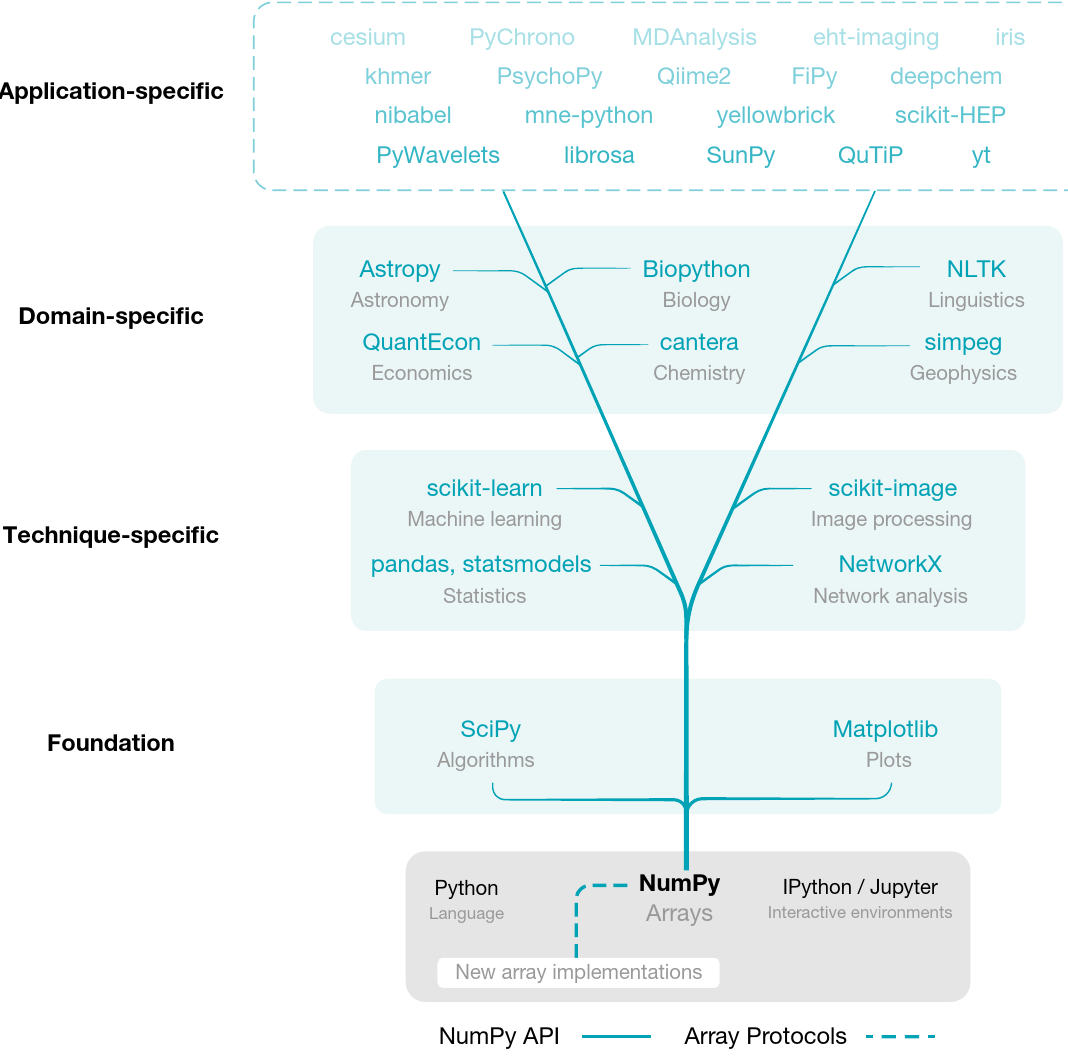
\includegraphics[scale=0.7]{fig/scipy-eco.png}
		\caption{The scientific Python eco-system}
		\label{fig:scipy}
	\end{figure}
	The picture \ref{fig:scipy} provides a glance at the huge system.\par

	The canonical implementation of NumPy stores the array in main memory and do computation on CPUs.
	As the problem size in research frontier continuse to grow, people find it hard
	to fit the data into single machine main memory and the power of CPUs are become insufficient.
	In deep-learning area, people are training networks with billions of paramters\cite{gpt3}.
	In seek for gravitational waves, Terabytes of data per data have to be examined\cite{gravwave}.
	To accomplish these challenging tasks, NumPy have to leverage modern specialized hardwares and explore parallism.
\end{newSec}

\begin{newSec}{The Legate NumPy System}
	\begin{newSubsec}{overview}
		Proposed and implemeneted by NVIDIA, Legate\cite{Legate} is a programming system that strives to accelerate NumPy programs with the power of GPUs and enable distributed computing.
		Normal NumPy codes are translated into the Legion\cite{Legion} programming model, which enhances the scalability and performance of programs.
		By offering interfaces mimics the NumPy array programming APIs and providing the equivalent semantics, Legate can achieve this while staying transparently to programmers.\par
		The benchmarks on machines with up to 1280 CPU cores and 256 GPUs show that Legate achieves weak-scalability with the state-of-the-art efficiency.
		Legate is capable for both constructing prototypes and scaling up pre-exists programs significantly.\par
		We will demonstrate the Legion programming model and how Python programs are translated into Legion.
	\end{newSubsec}

	\begin{newSubsec}{the Legion programming model}
		Designed as a programming model suitable for large scale high performance applications, Legion\cite{Legion}
		attach great importance on the locality and independence of data and tasks.
		Detailed summary on the data model and the task model, as well as the scheduling strategies are to be shown in this section.

		\subsubsection{Legion data model: the logical region}
		Reponsible for organizing all the long-lived data, logical regions is the a concept in Legion system.
		It is a 2D tabular where the rows are named by multi-dimensional coordinates and the columns are indexed by named fileds.
		This flexible data model gives Legion the power to manipulate N-dimensional arrays and crate arbitary views readily.
		The figure \ref{fig:logical-region} gives a brief example of the logical region.\par
		\begin{figure}[htbp]
			\centering
			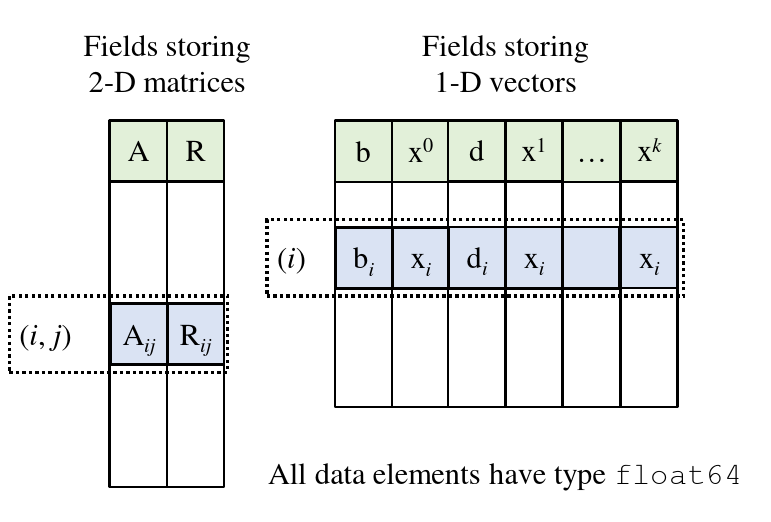
\includegraphics{fig/logical-region.png}
			\caption{{A example illustrating the logical region data model}\cite{Legate}}
			\label{fig:logical-region}
		\end{figure}
		Legion requires programers to declare the data locality and dependencies using logical regions.
		Moreover, every task, which will be covered later, has to specify the logical regions that are accessed,
		the access privilages (e.g., read-only, read-write or reduce) as well as the coherence (e.g., exclusive access and atomic access).\\
		Privileges provides the data dependence information of task, whichis used to extract potentially parallelism
		For example, if two tasks access the same region with read-only privilages the two tasks can potentially be run in parallel.
		The coherence configuration specifies the semantics of concurrent accesses.
		For example, if the program executes $f_1(r); f_2(r)$ where both tasks  declare exclusive access to $r$.
		Then Legion has to guarantee that the output of execution will be as if the program runs sequentially.
		On the other hand, if the tasks access $r$ with atomic coherence, then Legion guarantees that $f_1(r)$ runs
		entirely before  $f_2(r)$ or $f_2(r)$ runs before $f_1(r)$.\\
		\begin{figure}[htbp]
			\centering
			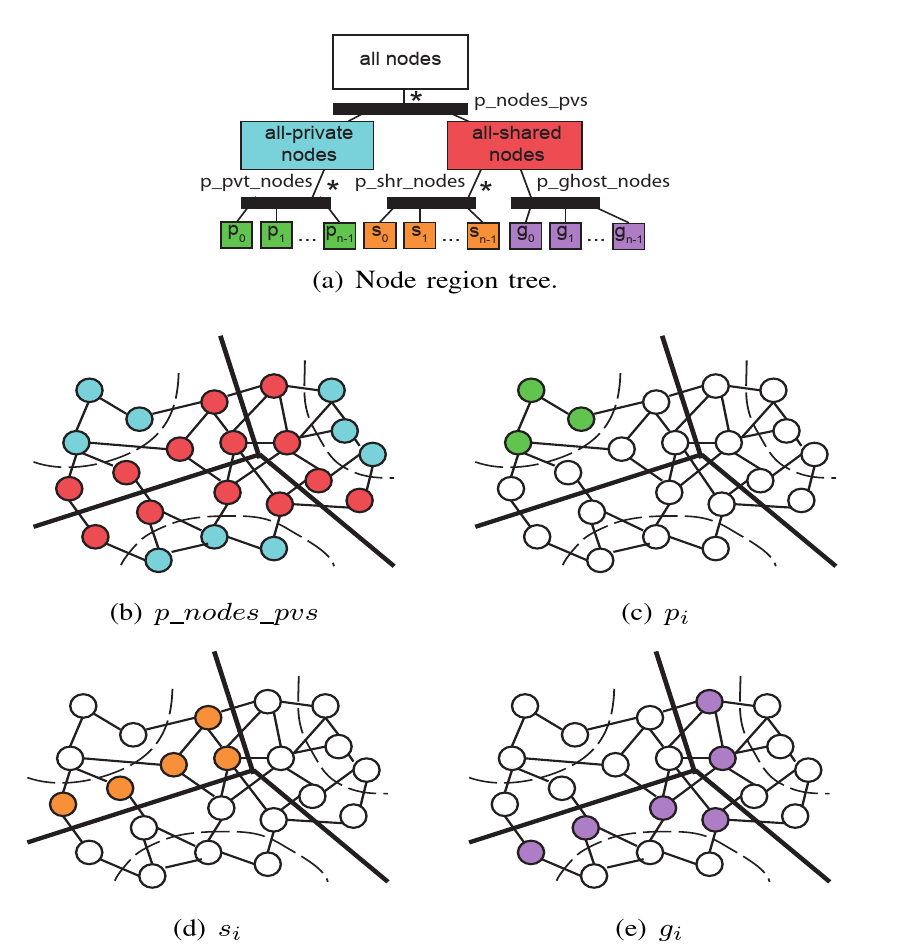
\includegraphics[scale=0.7]{fig/legion-partition.png}
			\caption{{A example of hierachical and natural decomposition}\cite{Legion}}
			\label{fig:region-tree}
		\end{figure}
		Although data access and coherence information are required to be given, programmers never specify the physical data layout, the runtime system handles data partition and distribution automatically, staying transparent to the logical data model of a programs.
		How the data are actually partitioned and distributed are not determined solely by the logical region structure,
		the hardware conditions and runtime behaviors are all taken into account.
		Both natural decomposition and hierachical decomposition are applied to reduced the data transfer traffic and the increase locality of memory access pattern \ref{fig:region-tree}
		\subsubsection{Legion execution model: the task tree and deferred execution}
		Next, we will take a look at the execution model of Legion.\par
		The computation unit of a Legion program is called task.
		A unique top-level task marks the start of the whole program.
		Every task is allowed to create arbitary number of subtasks, thus forming a rooted task tree.
		In previous section, we have mentioned that Legion requires data access permissions.
		The launched subtasks only have access to regions that can be accessed by its parent.
		Moreover, the privilages on a region should be compatible with its parent's.\par
		A asynchronous execution model is employed in Legion programming language.
		A task launch call returns immediately to the caller.
		The return values of tasks are wrapped in future (also called promise in some areas).
		The caller can examine whether the computation of the previously launched task has finished through the future object or wait explicitly until the future is resolved.
		A noticable feature of future object is that it can be passed to other tasks, enabling easy compositon of tasks.\\
		Based on the knowledge of which region a task will access, dynamic dependencies analysis at runtime determines the relationship between tasks.
		Tasks that are found to be independent can be re-ordered or executed in parallel while dependent data and tasks are handle with care to preserve the semantics of sequential execution order.
	\end{newSubsec}

	\begin{newSubsec}{logical regions for NumPy arrays}
		To translate NumPy \mintinline{python}{numpy.ndarray} into logical region, the most obvious way is to create a logical region for every array object in the Python program.
		However, this is not the way Legate do. Legate to pack multiple arrays of the same shape into a single region, where each column corresponds to an array.
		In the example of logical region \ref{fig:logical-region}, we can see that the arrays $b,x^0,x^1\ldots x^k$ are organized in one region.\\
		The motivation for packing several arrays in one region is to reduce the cost of dynamic partitioning.
		Suppose that we have two arrays of the same shape $x,y$, when perform element-wise operations e.g, $x+y$ adding two vectors or $x\cdot y$ computing dot-product,
		we would benefit from partitioning $x,y$ in exactly the same way.
		Thus, when performing operation $x+y$, the cost of dynamic partitioning is avoided.\par
		To create array slices for implementing the advanced indexing operations in NumPy, Legate calls Legion scatter and/or gather to copy from the original array.
		This reflect the semantics of array slicing: create a copy rather than an alias.\\
		\begin{figure}[htbp]
			\begin{center}
				\begin{subfigure}{0.4\textwidth}
					\centering
					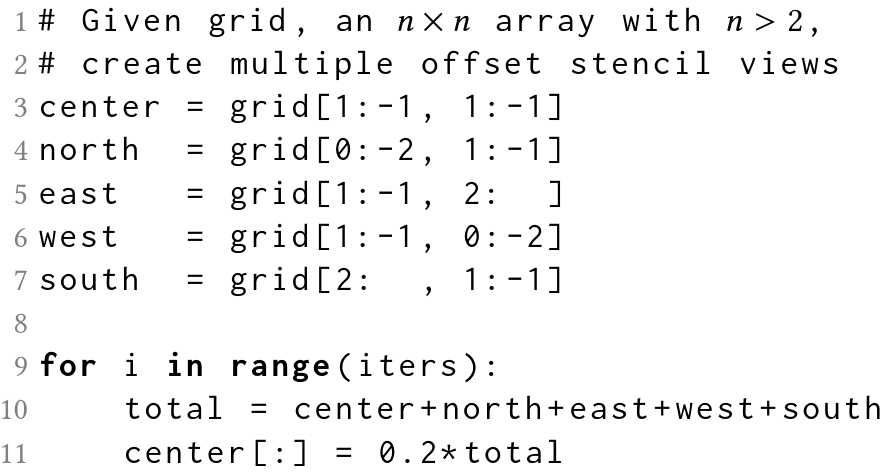
\includegraphics[scale=0.6]{fig/code-stencil.png}
					\caption{2D-stencil using basic indexing}
				\end{subfigure}
				\begin{subfigure}{0.4\textwidth}
					\centering
					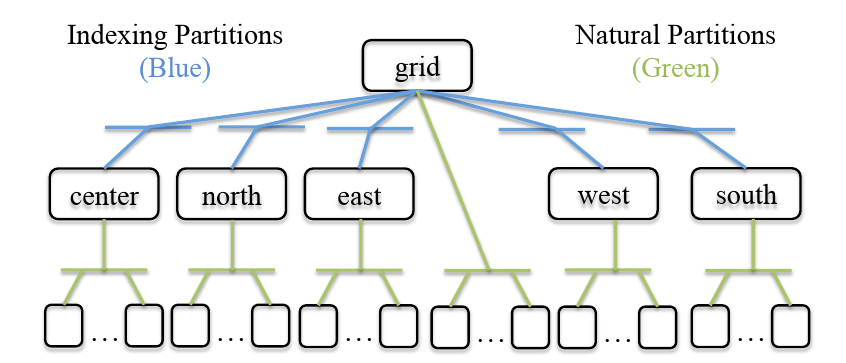
\includegraphics[scale=0.6]{fig/stencil-region.png}
					\caption{the region tree created by the stencil program}
				\end{subfigure}
			\end{center}
			\label{fig:basicindexing}
			\caption{illustration of basic-indexing in Legate}
		\end{figure}
	\end{newSubsec}
	In contrast, for basic indexing, which create views/reference to the original array instead of a copy,
	Legate simply create a sub-region from the logical of the orignal array.
	In Legion Sub-region are aliased to the ancestor regions (including the direct parent region).
	Here we give an easy-to-read example of basic indexing \ref{fig:basicindexing}.

	\begin{newSubsec}{legion tasks for NumPy APIs}
		Legate provides NumPy compatible APIs and implement them using Legion task, where each NumPy operation is decomposed into a few asynchronous tasks.
		When running the program, the tasks that implement N-dimensional array computations are created and submitted to the Legion runtime.\\
		Recall: Legion runtime, guided by a mapper, will handle region partitioning and task schedule.
		Therefore, Legate can focus purely on domain-specific partitioning and mapping of each task.
		semantics being transparent to the low-level details of distributed execution.\par

		Legate have registerd three different implementation variants for every NumPy operation,
		one sequential version for a single CPU core, one OpenMP version for a multi-core CPU, and CUDA version for NVIDIA GPU.\\
		To avoid code duplication and enable extensibility, Legate implement all the three task variants in one C++ template function.
		The generic template function can be instantiated using different executors.
		Executors, defined in the Agency library, are objects that specify the how the code can be executed. Agency library provides executor for CPUs, OpenMP and CUDA.\\
		This design allows programmer to extend Legate for utilizing alternative accelerators, all you need to do is simply to create a executor for that hardware accelerator.
	\end{newSubsec}

	\begin{newSubsec}{Legate mapper: domain-specified mapping and control replication}
		Legate translate Python NumPy operations into Legion programming model.
		Legion can handle the mapping and scheduling automatically, however it has no domain-specific heuristic.
		To achieve maximized performance, Legate implement a mapper to leverage its domain-specific knowledge of NumPy.\par

		\begin{figure}[htbp]
			\centering
			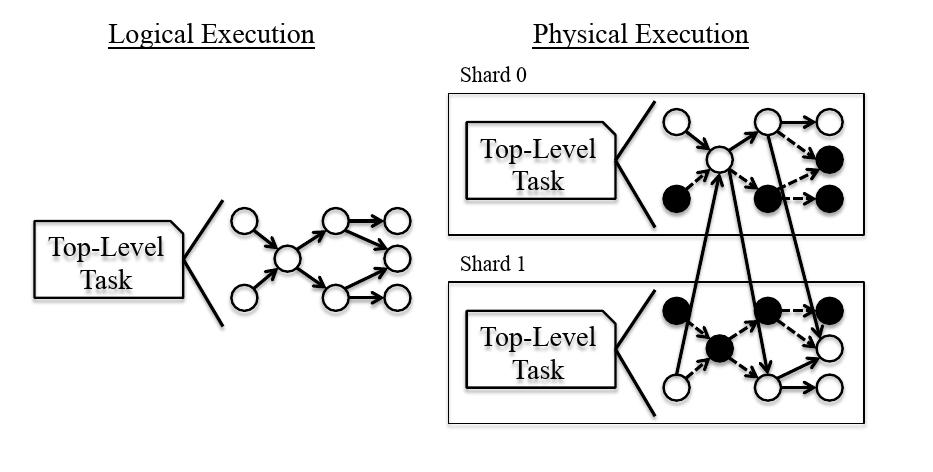
\includegraphics{fig/ctrl-repl.png}
			\caption{control replication}
			\label{fig:ctrlrepl}
		\end{figure}
		Recall that Legion programs start as a unique root task, the machine that initally runs this task can become a sequential bottleneck
		since it has to distribute large amount of sub-tasks to other nodes. This is quite common in systems that have a centralized controller
		which limit the scalability.\\
		Control replication is a feature in Legion runtime system designed address this problem.
		Multiple copies of a task are spawned on different machines, they work collectively to reduce the time waiting for dragger.\\
		The figure \ref{fig:ctrlrepl} gives an example on how control replication helps to scale-up a program.
	\end{newSubsec}

	\begin{newSubsec}{benchmarks}
		To make a empirical analysis on the scalability of Legate, they made a few representative benchmarks.
		The benchmarks are done on a cluster constists of 32 NVIDIA DGX-1V node.
		Each node is equipped with 8 Tesla V100 GPUs connected by a hybrid mesh cube topology using NVLink and PCI-E.
		The CPUs on the DGX-1V ndoe are two 20-core Intel Xeon E5-2698 CPUs with hyperthreading enabled and 256 GB of DDR4 memory.
		The Nodes in the cluster are connected by an Infiniband EDR switch with each node having 4 Infiniband 100 Gbps NICs.\\
		It turns out that Legate has obtained near linear efficiency weak-scaling with up to 1280 CPUs and 256 GPUs.

		\begin{figure}[htbp]
			\begin{subfigure}{0.5\textwidth}
				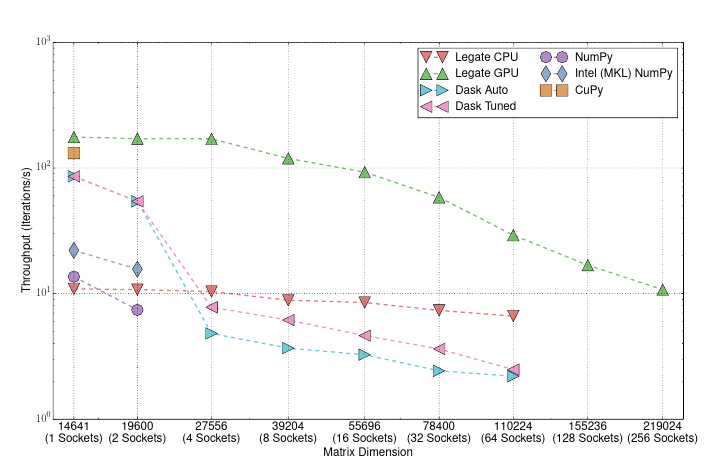
\includegraphics{fig/scale-CG.png}
				\caption{Weak-scaling of a preconditioned CG solver}
			\end{subfigure}
			\begin{subfigure}{0.5\textwidth}
				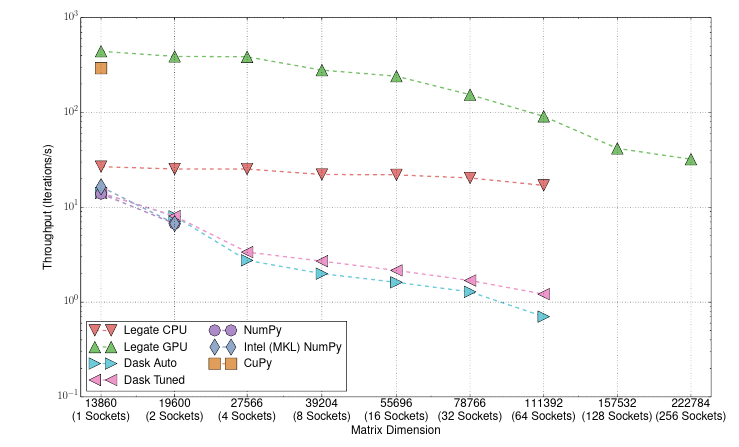
\includegraphics{fig/scale-jacobi.png}
				\caption{Weak-scaling throughput of a Jacobi solver}
			\end{subfigure}\\
			\begin{subfigure}{0.5\textwidth}
				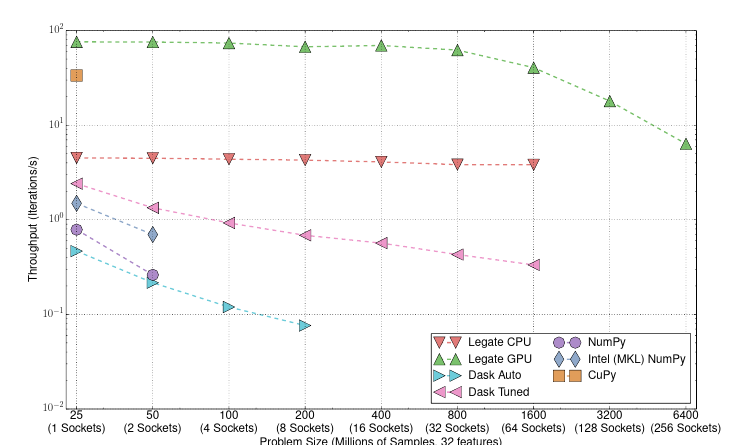
\includegraphics{fig/scale-logisticregression.png}
				\caption{Weak-scaling of a logistic regression}
			\end{subfigure}
			\begin{subfigure}{0.5\textwidth}
				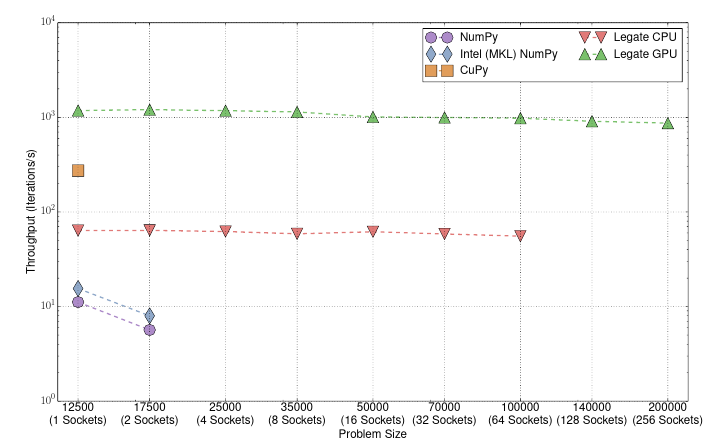
\includegraphics{fig/scale-stencil.png}
				\caption{Weak-scaling throughput of a 2D stencil}
			\end{subfigure}

			\label{fig:benchmarks}
			\caption{{the benchmarks result}\cite{Legate}}
		\end{figure}
	\end{newSubsec}
\end{newSec}

\begin{newSec}{Related Works}
	As we have mentioned in the introductory section, people have been trying to accelerate Python ever since the rise of data science.
	In this section, we are to cover a few more Python libraries/frameworks/runtimes/compilers for speeding up large scale data science applications.\par
	Only general purpose open source project are covered.
	In fact, a variety of domain-specified NumPy implementations do exists and a considerable number of enterprises have developed their own closed-source replacement of NumPy.
	\begin{newSubsec}{Theano / Aesara}
		Aiming at accelerating mathematical expressions, Theano\cite{Theano}, consisting of a set of NumPy-like APIs and a compiler.
		Before the Python code is executed, Theano compiler transform it into optimized high performance C++ code and link it as a dynamically loaded Python modules.\par
		Theano is the pioneer of differentiable programming paradigm, the auto symbolic differentiation features
		allow programmers to implement numerical optimization algorithm such as the gradient descent without manually evaluating the derivatives, which is painful and error-prone.
		This key feature not only alleviates manual symbolic calculation, but also opens a door for advanced code generation.
		Having full access to the computational graph, Theano applies local graph transformations to eliminate unnecessary, slow or numerically unstable expression patterns.\par
		Theano is orginally a research project from Google MILA groups, however MILA stopped the development and maintance in 2017.
		It is being continued as aesara, a community fork of Theano.
	\end{newSubsec}

	\begin{newSubsec}{Numba}
		Numba\cite{Numba} is similar to Theano, both libraries try to compile Python code into high performance. When comparing them, Numba is more powerful and flexible.\par
		To overcome the performance degrade of Python interpreter and take the advantage of parallel execution,
		the only modification needed is simply marking functions with \mintinline{Python}{@jit,@cuda.jit,@cfunc} decorator.
		The code then get transformed into optimized high performance code and can even utilize common hardware accelerators.\par
		Numba implement a JIT (just in time) compiler to transform normal Python code into LLVM IR.
		They do optimization on the LLVM IR level and generate machine code from it.
		The benefit of using LLVM IR is that Numba can support for targeting different hardwares such as multi-core CPUs, GPGPUs and Google TPUs.
	\end{newSubsec}


	\begin{newSubsec}{CuPy: array programming on a single NVIDIA GPU}
		Prior to the birth of Legate, the researchers at NVIDIA developed a drop-in replacement for NumPy called CuPy\cite{CuPy}.
		It is highly compatible with the N-dimensional array APIs provided by NumPy.
		Typically, to turn a CPU code into CUDA program can be achieve by replacing \mintinline{Python}{import NumPy as np} with \mintinline{Python}{import cupy as np}.\par
		CuPy does not simple move the data onto GPU main memory and implement array operations with CUDA kernels.
		It is linked with NVIDIA's CUDA toolkit. {cuBLAS, cuSOLVE, cuRAND, cuFFT} are integrated into CuPy.
		CuPy also include support low-level CUDA codes. User-defined CUDA kernels written in C++ are wrapped and loaded readily.
	\end{newSubsec}

	\begin{newSubsec}{Dask}
		The previous three libraries focus on single node performance boost,
		while Dask\cite{Dask} is targeted fully utilizing the power of multi-node cluster.
		Dask is a task-based runtime system for parallel and distributed computation.\par
		\mintinline{Python}{dask.array}, \mintinline{Python}{dask.bag} and \mintinline{Python}{dask.dataframe} are the three main data structure provided,
		programmer use the then to compose programs.
		Dask analysis the program and divides the computation into tasks.
		The tasks are organized in a DAG called \mintinline{Python}{dask graph}. The edges and vertices represent dependencies and computation tasks respectively.
		Dask explore the graph and schedule execution of tasks dynamically until completion.\par
		Dask provides richer data structures than Legate, however the performance is lower than Legate.
		In the Legate paper, researchers at NVIDIA compared the performance and scalability of Dask and Legate.
		They concluded that Legate outperforms Dask in the sense of absolute speedup and weak-scalability.
	\end{newSubsec}

	\begin{newSubsec}{Tensorflow, PyTorch and MXNet}
		The last five years have witnessed the tide of deep learning.
		As the typical size of neural networks grows, training and inference require more computation power and memory foodprint.\par
		Tensorflow, PyTorch and MXNet are three popular deep learning frameworks, each has implemented tensor (which is a fancier name for ndarray) facilities on GPU.
	\end{newSubsec}
\end{newSec}

\begin{newSecNoNP}{Conclusion}
	In this paper review project, we give an anatomy of the Legate system, a NVIDIA research project provides accelerated NumPy-compatible N-dimensional array operations on distributed GPU cluster.\par
	In the beginning we give a overview of the scientific Python ecosystem, where NumPy plays a central role.
	We then explored the Legion runtime upon which the Legate is built.
	Shortly after that, we presented a detailed explanation on how Legate maps NumPy data structures and computational task into Legion data and tasks.\par
	In the last part, we covered several related works.
	We give a short summary on their mechanism and compared them with Legate.
\end{newSecNoNP}
\printbibliography{}
\appendix

\begin{newSec}{Sample code}
	\begin{newSubsec}{NumPy and Legate}
		It is convenient to express matrix operations in NumPy API. Here we illustrate how to implement Jacobi iteration with NumPy.
		\inputminted{python}{src/numpy.py}
	\end{newSubsec}
	\begin{newSubsec}{Theano/Aesara}
		Here we demonstrate how to implement \href{https://aesara.readthedocs.io/en/latest/tutorial/examples.html#a-real-example-logistic-regression}{logistic regression} in aesara.
		\inputminted{python}{src/theano.py}
	\end{newSubsec}
	\begin{newSubsec}{Numba}
		The following code gives a simple example on numba's JIT decorator.
		\inputminted{python}{src/numba.py}
	\end{newSubsec}
	\begin{newSubsec}{CuPy}
		With CuPy, one can speedup common scientific computation task with NVIDIA CUDA toolkit.
		We demonstrate how to use cuFFT.
		\inputminted{python}{src/cupy.py}
	\end{newSubsec}
\end{newSec}


\end{document}
